%                                                                 aa.dem
% AA vers. 9.1, LaTeX class for Astronomy & Astrophysics
% demonstration file
%                                                       (c) EDP Sciences
%-----------------------------------------------------------------------
%
%\documentclass[referee]{aa} % for a referee version
%\documentclass[onecolumn]{aa} % for a paper on 1 column  
%\documentclass[longauth]{aa} % for the long lists of affiliations 
%\documentclass[letter]{aa} % for the letters 
%\documentclass[bibyear]{aa} % if the references are not structured 
%                              according to the author-year natbib style

%
\documentclass{aa}  

%
\usepackage{txfonts}
\usepackage{makeidx}         % allows index generation
\usepackage{listings}	%Format Listings properly
\usepackage{lipsum}    %Blindtext
\usepackage{graphicx} % use various graphics formats
\usepackage[german]{varioref} 	% nicer references \vref
\usepackage{caption}	%better Captions
\usepackage{booktabs} %nicer Tabs
\usepackage{array}
\usepackage{chngcntr}
\usepackage[hidelinks=true]{hyperref} % keine roten Markierungen bei Links
\usepackage{fnpct} % Correct superscripts 
\usepackage[T1]{fontenc}
\usepackage[utf8]{inputenc}
\usepackage{calc} % Used for extra space below footsepline
\usepackage{acronym}
\usepackage{algorithm}
\usepackage{algpseudocode}
\usepackage[ngerman]
%%%%%%%%%%%%%%%%%%%%%%%%%%%%%%%%%%%%%%%%

%%%%%%%%%%%%%%%%%%%%%%%%%%%%%%%%%%%%%%%%
%\usepackage[options]{hyperref}
% To add links in your PDF file, use the package "hyperref"
% with options according to your LaTeX or PDFLaTeX drivers.
%
\begin{document} 

   \title{Projektreport}

   \subtitle{Aunt Elisa}

   \author{Johannes Deufel, Jannik Fischer, Simone Marx und Simon Scapan}

   \institute{Duale Hochschule Baden-Württemberg Mannheim, Coblitzallee 1-9, 68163 Mannheim}

   \date{Abgabe 17. Juli 2020}

% \abstract{}{}{}{}{} 
% 5 {} token are mandatory
 
  \abstract{In diesem Projektreport wird die Entwicklung eines Chatbots beschrieben, der besonders in der Zeit des Coronavirus zu weniger Einsamkeit unter isolierten Personen führen soll. Der Chatbot eignet sich dabei hervorragend für sogenannten Smalltalk, da die verwendete Seq2Seq-Technologie unter Einsatz von Recurrent Neural Networks (RNN) eine passende Antwort individuell auf Basis der eingegebenen Worte berechnet. Dieser Report enthält dabei sowohl wirtschaftliche Kalkulationen zur Umsetzung des Projekts, bereits bestehende wissenschaftliche Erkenntnisse zum Thema, konkrete Implementierungsansätze, als auch die erzielten Ergebnisse und eine kritische Bewertung dieser. Das gesamte Projekt findet sich in einem \href{https://github.com/SimonScapan/AuntElisa}{Repository auf GitHub}. \cite[Vgl.]{auntelisa}}
   \keywords{Seq2Seq --
                Chatbot --
                RNN
               }

   \maketitle
%
%-------------------------------------------------------------------

\section{Einleitung}
     Der Mensch ist ein soziales Wesen, welches stets bemüht ist, in einer Gruppe zu agieren. Durch die globale Pandemie des Coronavirus stellen die Regierungen vieler Staaten drastische Maßnahmen. Um das Virus einzudämmen,  wird die Bevölkerung angehalten, soziale Kontakte zu meiden. Vor allem Rentner und pflegebedürftige Menschen leiden an den Folgen des "Social Distancing", da diese als Risikogruppen ihre sozialen Kontakte auf ein Minimum reduzieren müssen. Es ergibt sich eine Marktlücke bei älteren Menschen, welche menschliche Kontakte haben möchten, jedoch wegen des Virus keine Möglichkeit mehr dazu haben. Um die Situation bei den betroffenen Personen zu verbessern, soll ein Chatbot entwickelt werden. Damit dieser bei der Zielgruppe gut vermarktet werden kann, ist es wichtig, dass die Anwendung einfach zu bedienen ist. Da in der Zielgruppe noch ein geringes Verständnis von technischen Anwendungen bzw. sogar eine Hemmschwelle herrscht, soll die Distribution vorwiegend über Business Customers, also über Pflegeheime geschehen. Ein umfassender Marketing Mix ist in Abbildung \ref{fig:Marketing_Mix} dargestellt. Der Chatbot soll dabei über maschinelles Lernen sinnvolle Antworten auf die kurzen sprachlichen Konversationen des Users geben. Auch aus wirtschaftlichen Gesichtspunkten ist es wichtig, die Anwendung möglichst kostengünstig anzubieten und dennoch einen angemessenen Gewinn zu erwirtschaften. Um dies zu erreichen, wurde kalkulatorisch ermittelt, welche Entwicklungskosten und laufende Kosten, sowie Erträge bei dem Projekt anfallen würden, wenn das Produkt mit 10 Euro für Endkunden und 50 Euro für Businesskunden bepreist ist (Abbildung \ref{fig:Ertrag_Jahr01}). In Abbildung \ref{fig:Langzeitertrag} wurde überprüft, ob das Projekt auch auf langfristige Sicht einen ausreichenden Ertrag erwirtschaftet.\\
      Der vorliegende Projektbericht beschreibt das wissenschaftliche Vorgehen bei der Durchführung des Projektes "Aunt Elisa". Nachfolgend wird sowohl auf bereits existierende wissenschaftliche Werke im Bereich der Chatbots eingegangen, als auch die verwendeten Methoden und Bibliotheken empirisch untersucht. Zudem werden auch die Ergebnisse vorgestellt und kritisch hinterfragt.
       
\section{Related Work}
    Es existiert verschiedenste Literatur, die auf die Hintergründe und die Funktionen der verschiedenen Methoden der Computerlinguistik eingehen und diese erforschen.\\
    Wie im folgenden Kapitel dargelegt, konzentriert sich diese Arbeit insbesondere mit der Anwendung von Deep Learning in diesem Bereich. Trotzdem sei angemerkt: \cite{bird} beschäftigt sich ausführlich mit den Möglichkeiten, die andere Methoden der Computerlinguistik beispielsweise unter Anwendung von Entscheidungsbäumen und des Naïve Bayes Klassifikators bieten.\\
    Die Literatur zu diesem Thema im Bereich Deep Learning geht auf verschiedene Algorithmen ein. Ganz besonders wird hier das Thema Seq2Seq beschrieben, was den Prozess beschreibt, einer Sequenz von Worten eine bestimmte weitere Wortsequenz zuzuordnen, die im Falle des Chatbots die automatisch generierte Antwort auf die eingegangene Nachricht darstellt. \cite[Vgl.][S.~1219]{jackson} Um dieses Konzept umzusetzen, wird sehr häufig auf ein Word2Vec-Modell zurückgegriffen, welches die Inputfeatures des neuronalen Netzes darstellt. Der sogenannte Wortvektor soll dabei den Kontext jedes Wortes wiedergeben, indem umliegende Wörter betrachtet werden. \cite[Vgl.][S.~1220]{jackson} Zur Umsetzung des Seq2Seq-Modells werden heutzutage in den meisten Fällen Recurrent Neural Networks angewandt. Diese eignen sich besonders gut, da hier die Ausgabe des aktuellen Schritts gleichzeitig die Eingabe für den nächsten Schritt ist. Die vorherigen Berechnungen werden also immer wieder in die Berechnung miteinbezogen. \cite[Vgl.]{koehrsen} Abbildung \ref{fig:rnn} verdeutlicht dabei die Funktionsweise eines Recurrent Neural Networks, indem es die wiederkehrende Schleife entfaltet und zeigt, dass jeder Schritt sowohl die vorherige Ausgabe, als auch ein neues Wort als Eingabe für die weitere Berechnung nutzt. So kann vereinfacht gesagt der Kontext der zuvor vorausgesagten Worte genutzt werden, um den Satz darauf basierend weiter aufzubauen. In vielen Fällen wird zusätzlich Teacher Forcing in einem Recurrent Neural Network verwendet, um die Eingaben durch vorherige Schritte zu verbessern und das Training so schneller konvergieren zu lassen.
    
\section{Verwendete Technologien und Bibliotheken}
    Dieser Abschnitt gibt einen Einblick in die verwendeten Technologien und Ideen zum Projekt, mit Schwerpunkt auf dem letztendlich verwendeten Ansatz. Es werden aber auch in Teilen verworfene Ideen beschrieben.
    \subsection{Systemarchitektur}
    
        Die Systemarchitektur ist wie in Abbildung   \ref{fig:Systemarchitektur} zu sehen aufgebaut. Sie besteht aus einem Client, dem React Frontend, einer Verbindung zum Backend via Flask und Python als Backend, welches den Chatbot beherbergt.\\
        Der Client setzt eine Anfrage ab, welche er in gesprochener Sprache an das React Frontend sendet. Das Frontend empfängt die Anfrage und verarbeitet zuerst die Sprache und konvertiert diese Mithilfe von Mozilla SpeechRecognition \cite[Vgl.]{mozilla20} in einen String. Da ein String einfacher in der Handhabung ist als ein Soundfile, welches weiter verarbeitet wird. Der erzeugte String wird dann über die Backendconnection an das Backend gereicht. Hier wird es dem Chatbot übergeben. Dieser verarbeitet den Input und erzeugt einen Output, welcher wieder zurück an das Frontend gereicht wird. Im Frontend wird dieser String nun mit SpeechSynthesis \cite[Vgl.]{mozilla19} als Audio Feedback an den User zurück gegeben.\\
        Unterstützt wird die Systemarchitektur von Docker. Das Projekt ist in zwei Container aufgeteilt, Frontend und Backend. Der Frontend Container kann auf dem Port 3000 und der Backend Container auf Port 5000 angesprochen werden. Zum Starten des Systems wurde eine Docker-Compose Datei hinzugefügt, welche beide Container erstellt und lädt. Um die Software nutzen zu können, muss man lediglich den Docker-Compose im Wurzelverzeichnis erzeugen und starten. Näheres ist dem Readme  \cite[Vgl.]{auntelisa} oder dem Anhang zu entnehmen.
    
    \subsection{Frontend}
        Das Frontend wurde auf der Basis von React aufgebaut. React bietet eine Grundstruktur und eine Lauffähige Webapplikation. Die Struktur des Frontend bei dieser Anwendung ist einfach gehalten. Sie besteht aus der Wurzel (App.js) und den beiden zweigen Chatbot und Landingpage. Die Landingpage beinhaltet die Startseite samt animiertem Logo und einer Schaltfläche, die einen zur Seite Chatbot umleitet. Hier hat man zwei Schaltflächen: Eine um eine Anfrage in Sprachform einzugeben und eine um die Antwort des Chatbots zu erhalten. Der Datentransfer zum Backend wird über die Datei Backendconnection realisiert.
        
    \subsection{Backend}\label{sec:backend}
        Grundsätzlich steht zu Beginn die Frage nach dem zu verwendenden Framework. Bei diesem Projekt fiel die Entscheidung diesbezüglich  auf Tensorflow. Diese initiale Entscheidung war vor allem durch persönliche Vorkenntnisse in diesem Bereich und den intuitiven Griff zum bekannteren geprägt. Darüber hinaus gestaltete sich die Suche nach Referenzprojekten mit diesem Framework als einfacher, als nach Projekten, welche Pytorch verwenden. Durch die Grundsatzentscheidung, die bestehende Implementierung von Seq2Seq in Tensorflow nicht zu verwenden, stellte sich die Frage, durch welche Technologien das Modell bestmöglich zu implementieren ist. Im Zuge dieser Recherche wurde sich dann für Keras als Erweiterung zu Tensorflow entschieden. Das Debugging bei Keras ist zum einen angenehmer. Zum anderen scheint Keras dabei deutlich intuitiver anwendbar und liefert eine Lösung, ohne zu komplexe Methoden zu verwenden. \\
        Als Basis dieser Frameworks fungieren einige verbreitete Python Librarys, die grundsätzliche Operationen in diesem Projekt unterstützen: numpy, os, pickle, random, statistics, sys, re, time, csv und  matplotlib. \\
        Üblich ist es für Projekte dieser Art, den Cornell Movie Dialogue Corpus zu verwenden.Oft werden auch für weniger ausführliche Projekte beziehungsweise Projekte mit anderen Anwendungsschwerpunkten andere Datensätze verwendet, für unseren allgemeinen Usecase ist der Cornell Movie Dialogue Corpus jedoch völlig ausreichend. Er enthält über 300.000 Gespräche zwischen ca. 9.000 Personen aus 617 Filmen. Durch diese relativ große Datenmenge und die breite Fächerung der Gespräche und Gesprächspartner eignet sich der Datensatz hervorragend für dieses Projekt. \\
        Im Preprocessing wurde dieser Datensatz so aufbereitet, dass er für das Folgende Training, Testing und die Validierung geeignet ist. Dabei wurden der Text normalisiert, indem Sonderzeichen entfernt, alle zusammengesetzten Worte wie "you're" durch ihr Pendant, hier "you are" und alle Großbuchstaben durch die entsprechenden Kleinbuchstaben ersetzt wurden. Anschließend werden zu lange Sätze aus dem Datenbestand entfernt. Dann wird ein Dictionary mit jedem Wort und der dazugehörigen ID und ein Dictionary mit ID und dem entsprechenden Wort gebildet. Aus den bereinigten Gesprächen werden Message-Response-Paare in einer Liste gebildet, bei dem an jede Message und jede Response eine Start- und einen Endtoken am Anfang bzw. Ende angefügt werden. \\
        Im Training werden zunächst die Hyperparameter bestimmt und die vorverarbeiteten Daten geladen. Dort wird zunächst ein Split der Daten vorgenommen: 70\% Training, 5\% Testdaten und 15\% Validierungsdaten. Dann wird eine Embeddingmatrix aus dem zuvor definierten Vokabeldictionary erstellt, die die verschiedenen Worte und ihre Beziehungen zueinander in einer Matrix darstellt. Die darin enthaltenen Worte werden durch Vektoren eines mehrdimensionalen Raums repräsentiert, über welche auch ihre Ähnlichkeit bestimmt wird. Diese Embeddingmatrix wird im Training durch vortrainierte Wordvektoren, sogenannte "GloVe" unterstützt.
        Danach werden die Encoder- und Decoder-Klassen des Modells initiiert. Der Encoder enthält dabei bidirektionale LSTM Layer, um  einen Datenfluss in beide Richtungen zu ermöglichen und dem RNN ein "Gedächtnis" zu geben. Dieser Sachverhalt ist in Abbildung \ref{fig:lstm} visualisiert. Zusätzlich wird die Methode dropout verwendet, um Overfitting zu verhindern und die Performance zu steigern.
        Der Decoder besteht aus Dense- und GRU-Layern und wird durch das Konzept der Attention unterstützt, um die Ergebnisse zu verbessern. Dense-Layers werden in diesem Projekt regulär dafür genutzt, ihren jeweiligen Input mit den gegebenen Gewichten aus der Embeddingmatrix zu verrechnen. Die GRU-Layer kreieren seitens des Decoders eine Art "Kurzzeitgedächtnis" und verarbeiten über sogenannte „update and reset gates“ nicht nur die aktuellen Informationen, sondern erhalten ähnlich wie die LSTM-Layer auch ältere Informationen. Die Attention unterstützt den Decoder, indem sie ebenfalls eine Art Kurzzeitgedächtnis pro Iteration erstellt und die Eigenheiten der Wortreihenfolge der vorgegebenen Sprache analysiert. So trägt sie zu einer natürlicheren Bildung der Outputs bei. 
        In diesem Projekt wird der Adam-Optimizer verwendet, um global die Gewichte des RNN upzudaten.
        Durch die Nutzung der Colaboratory-Ressourcen von Google und auch zur Validierung wird das Modell nach jeder Epoche zwischengespeichert, und bei bedarf an der letzten Stelle wieder aufgerufen.
        Pro Trainingsepoche werden nach der vorangegangenen Initialisierung der Methoden die Message-Response-Paare nach Message und Respone geteilt und die jeweiligen Wörter durch ihre Indizes ersetzt. Zudem wird die Länge der jeweiligen Sätze auf 20 Wörter genormt und bei bedarf durch das so genannte Padding mit Nullen aufgefüllt. Die Sätze werden in Listen für den Encoder beziehungsweise Decoder geschrieben, bis diese Listen die passende Größe für einen Schritt basierend auf einer Mini-Batch des Training erreicht haben. Die Encoder und Decoder Listen werden dann dem RNN übergeben und durch dieses verarbeitet. Zum Verfolgen des Lernfortschritts wird für jeden Batch der Verlust (das Loss) berechnet, indem die erwartete Response mit der Response des Datensatzes abgeglichen wird. Dieses Loss wird über die jeweiligen Mini-Batches aufsummiert, um das durchschnittliche Loss pro Epoche zu berechnen. Es wird ebenfalls immer das beste Epochenloss, sowie die Entwicklung dessen gespeichert. 
        Nach jeder Epoche wird die beste Epoche mit dem zugehörigen Loss, der Berechnungszeit pro Epoche und immer die selben fünf Testsätze für eine qualitative Überprüfung mit den berechneten Antworten ausgegeben. Zusätzlich wird nach jeder dritten Epoche ein Schaubild der Entwicklung des Loss ausgegeben.\\
        Innerhalb dieses Projekts wurden 200 Epochen trainiert und über den Test die optimale Epoche dieser für die Anwendung gewählt. Der Test ist genauer im Anhang erläutert.\\
        Bei Interaktion durch den Anwender wird die Spracheingabe durch das Frontend wie beschrieben dem Chatbot übergeben. Dieser generiert dann auf Grundlage des angehängten Modells und des RNN eine Response, welche dem Frontend zurückgegeben wird und dann als normalsprachliche Response ausgegeben wird.
        
    
    \subsection{Verworfene Ansätze}
        Die folgenden Teilabschnitte befassen sich mit Ansätzen, welche im laufe der Entwicklung des Projekts aufgekommen und nach intensiver Prüfung aus verschiedenen Gründen nicht weiter verfolgt wurden.
        \subsubsection{Deep Learning}
            Die ersten Implementierungsversuche im Rahmen des Data Exploration Projects wurden nach einer ausgiebigen Recherche durch gezielte Beispielsuchen stark beeinflusst. Dabei war es das Ziel, sich mit verschiedenen Implementierungsmöglichkeiten auseinanderzusetzen und zunächst Erfahrungen durch Anpassung bereits bestehender Modelle zu sammeln. Das Data Preprocessing wurde dabei in jedem Fall selbst geschrieben und je nach Modell angepasst, um die verschiedenen Modelle bestmöglich bewerten zu können.\\
            Das erste konkrete Modell, mit dessen Lauffähigkeit und Funktionalitäten sich befasst wurde, ist auf \href{https://github.com/tensorlayer/seq2seq-chatbot}{GitHub} zu finden. \cite[Vgl.]{tensorlayer} Der Autor hat dabei die bereits implementierte Seq2Seq Funktion aus Tensorflow angewandt und dadurch ein lauffähiges Modell erstellt. Es war uns dabei möglich, ein passendes Preprocessing zu programmieren, und nach einigen Anpassungen das Modell zu trainieren. Bis Epoche 29 verbesserte sich das Modell dabei stetig. Ab Epoche 30 gab es jedoch ein Problem mit den Wahrscheinlichkeiten (Weights), die plötzlich nicht mehr ausschließlich positiv waren. Somit konnte das Modell nicht mehr weiter trainieren. Es war leider im Rahmen unserer Möglichkeiten nicht möglich, diesen Fehler zu beheben. Zudem war das Modell der Epoche 29 noch nicht zufriedenstellend, sodass eine alternative Lösung gefunden werden musste. Um diesen Ansatz trotzdem zu dokumentieren, ist auch diese Version als Model 1 im zu dieser Arbeit gehörenden Repository zu finden.\\
            Das zweite Modell, mit dem sich befasst wurde, ist auf \href{https://towardsdatascience.com/how-to-implement-seq2seq-lstm-model-in-keras-shortcutnlp-6f355f3e5639}{Towards Data Science} zu finden. \cite[Vgl.]{takezawa} In dieser Implementierung wurde keine vorab gebaute Funktion verwendet, sondern ein RNN eigenständig definiert. Dies entsprach auch eher den Vorstellungen einer Modellimplementierung für das Data Exploration Project. Nach diesem Vorbild wurde versucht, ebenfalls ein Seq2Seq Modell durch ein RNN selbst zu implementieren. Dafür war es nötig, verschiedene Layer zu definieren. Wichtig dabei ist vor allem die Definition und Verbindung der verschiedenen Layer. Dabei sind große Probleme aufgetreten, wodurch das Training nicht lauffähig war und kein Modell erstellt werden konnte. Konkret waren dabei die Input- und Outputdimensionen der Layer problematisch. Dieser Fehler konnte ebenfalls nicht behoben werden, daher wurde die dritte und letztlich erfolgreiche Implementierungsmöglichkeit angestrebt, die unter \ref{sec:backend} auf Seite \pageref{sec:backend} bereits genauer erläutert wurde.\\
            
        \subsubsection{Alternative Methoden der Computerlinguistik}
            In der Computerlinguistik bestehen zur Implementierung eines Sprachbots neben des verwendeten Deep-Learning Ansatzes weitere Methoden, die den Sinn der Computerlinguistik, in diesem Falle, die Eingabesequenz in allen Einzelheiten zu verstehen und genauso zu reagieren wie ein Mensch \cite[Vgl.][S.~16]{goyal}, verfolgen. So bieten sich beispielsweise ein Naive Bayes Klassifikator oder ein Entscheidungsbaum an, der durch die Struktur des Wortes die jeweilige Wortart erkennt \cite[Vgl.][S.~245]{bird}. Darauf basierend kann im weiteren Verlauf der Verarbeitung der Sequenz beispielsweise mit einer vereinheitlichten Struktur gearbeitet werden. Unter genauerer Betrachtung der nötigen Methoden fällt jedoch auf, dass zahlreiche alternative Methoden notwendig sind, um nur mit jenen den Inhalt einer Sequenz zu extrahieren und dabei auf ein vergleichbares Ergebnis zu gelangen, wie es unter Verwendung des Deep-Learning Ansatzes der Fall wäre. Zudem bräuchte es einen sehr großen vielfach gelabelten Datensatz, um die einzelnen Modelle zu trainieren, was wiederum mit Hilfe von Deep-Learning wesentlich einfacher umgesetzt werden kann, da hier nur ein Datensatz mit einem Label, nämlich Frage oder Antwort benötigt wird. Dies sind Gründe, weshalb in dieser Arbeit stattdessen mit den Deep-Learning Methoden gearbeitet wird.

\section{Ergebnisse}
    Ergebnis dieses Projektes sind zwei technisch verschiedene Modelle. Ersteres erzielt dabei weniger sinnvolle Ergebnisse, was letztendlich auf den Verzicht vortrainierter Word-Embeddings zurückzuführen ist, aber auch mit dem frühen Abbruch des Trainings wegen negativer Wahrscheinlichkeiten zusammenhängt. Eine quantitative Messung der Ergebnisse dieses Modells erfolgte jedoch nicht, da schon ein einfacher Blick auf die Ergebnisse genügt, um festzustellen, dass die vorhergesagten Antworten weder inhaltlich sinnvoll sind, noch grammatikalischen Regeln folgen.\\
    Auf der anderen Seite steht das Modell, welches schließlich in die finale Anwendung eingebunden wurde. Dieses basiert auf vortrainierten Word-Embeddings, um sinnvolle Ergebnisse mit weniger Rechenaufwand zu erzielen. Für jede Epoche dieses Modells wurde ein Verlust auf Basis der Trainingsdaten berechnet. In Abbildung \ref{fig:model} wird der Verlust jeder Epoche durch die blaue Linie repräsentiert. Der Verlust stellt hier den zu minimierenden Fehler da. Wird der Verlust anfangs noch stark reduziert, flacht die Kurve zwischen Epoche 60 und 80 deutlich ab. Hier ist eine nahezu kontinuierliche Verbesserung der Ergebnisse zu erkennen. Basierend auf den Trainingsdaten könnte demnach die zuletzt trainierte Epoche 200 verwendet werden, da diese eindeutig den besten Verlust erzielt. Es scheint sogar, als könnte fortlaufend weiter trainiert und somit stetig bessere Ergebnisse erzielt werden. Tatsächlich muss ein Modell aber auf neuen Daten getestet werden, die vorher nicht für das Training verwendet wurden. Aus technischen Gründen wurde für den Test ein anderes Maß verwendet, was die Vergleichbarkeit zwischen Test und Training zwar mindert, aber die Testergebnisse unter den Epochen miteinander vergleichen lässt. Da genau diese Eigenschaft für die Wahl der besten Epoche notwendig ist, wird für den Test auf ein Ähnlichkeitsmaß zurückgegriffen: die Cosine-Similarity \eqref{eq:similarity}. Weisen die echte Antwort und die durch das Modell vorhergesagte Antwort auf eine Nachricht eine sehr hohe Ähnlichkeit auf, nimmt die Cosine-Similarity den Wert eins an. Sind die Sätze komplett verschieden, ergibt die Cosine-Similarity null. So wurde für alle Testdaten eine Ähnlichkeit ermittelt und daraus der Mittelwert berechnet. So wird jede getestete Epoche durch einen Ähnlichkeitswert repräsentiert, der möglichst hoch sein sollte. Dieser Wert wurde auf Grund des hohen Rechenaufwands nur für jede zwanzigste Epoche ermittelt. Das Ergebnis wird durch die rote Linie in Abbildung \ref{fig:model} dargestellt. Da ein möglichst hoher Ähnlichkeitswert erzielt werden soll, wurde Epoche 120 als die optimale Epoche identifiziert. Zwar erzielen einige der vorherigen Epochen bessere Werte, jedoch liegt das daran, dass diese besonders häufige Wörter vorhersagen und in einem qualitativen Test durchfallen würden, da die Satzstruktur und Vielfalt hier nicht gegeben sind. Daher muss sich auf fortgeschrittenere Epochen konzentriert werden, wovon Epoche 120 die maximale Similarity von 7,2 \% erzielt und diese daher auch in der Anwendung eingebunden ist.
    
\section{Bewertung der Ergebnisse}
    Neben der Erzielung eines recht niedrigen Wertes der Cosine-Similarity, wird auch rein intuitiv während der Nutzung des final eingebunden Chatbots deutlich, dass viele der Antworten durchaus sinnvoll sind und zumindest für den sogenannten Smalltalk genügen könnten. Fachlich tiefgehendere und zusammenhängende Gespräche sind mit diesem Modell jedoch noch nicht möglich, wird die Antwort doch lediglich auf Basis der Wörter der Eingangssequenz berechnet und ist somit stark von den vorherigen Trainingsdaten abhängig. Ein Training über die genutzte Epoche 120 hinaus führt dabei lediglich zu einem sogenannten Overfitting, da sich das Modell so nur noch stärker auf die Eigenheiten der Trainingsdaten anpasst, diese aber nicht für Testdaten gelten und somit die Cosine-Similarity wieder allmählich sinkt.\\
    Eine weitere Verbesserung des Ergebnisses könnte durch eine ausführlichere Validierung der Hyperparameter erzielt werden. So könnten hier weitere Parameter wie die Anzahl der Epochen, Layer und die zugelassene maximale Satzlänge vorab validiert werden. Zudem kann es sich vorteilhaft auf das Ergebnis  auswirken, die Zahl an Kombinationen und Ausprägungen im Sinne des Grid-Search-Algorithmus zu erhöhen, wodurch die Wahrscheinlichkeit, die optimalen Hyperparameter zu finden, erheblich steigt. Aus Gründen der Knappheit an Zeit und Ressourcen konnte nur eine begrenzte Auswahl an Kombinationen validiert und nicht die optimale der hier ermittelten Kombinationen im Training verwendet werden. Natürlich führt dieser Umstand zu Einbußen in der Qualität des Modells, welche aber aufgrund der insgesamt guten Ergebnisse vernachlässigt werden können.\\
    Des weiteren wurden für das Training bereits einige vorab trainierte Word-Embeddings verwendet, die insgesamt für ein besseres Ergebnis sorgen. Hierbei muss beachtet werden, dass diese von Dritten stammen. Ihre Nutzung ist aber gerechtfertigt, besonders im Hinblick auf einen Vergleich zum ersten verworfenen Modell, welches deutlich schlechtere Ergebnisse erzielt hat, auch wenn für dieses kein quantifizierter Test erfolgte. Da aber all die zusätzlichen Wörter und das Seq2Seq-Modell ohne vorab trainierte Datensätze entstanden, kann das hier trainierte Modell trotzdem als Erfolg gewertet werden.\\
    Unabhängig des Modells bietet die Webanwendung zwar alle Funktionalitäten, um das Programm vollkommen funktionsfähig auszuführen, jedoch gelang die Steuerung doch nicht so intuitiv wie erhofft. Dies liegt vor allem daran, dass der perfekte Zeitpunkt für die Spracheingabe von einem roten Recording-Symbol im Tab-Fenster des Browsers abhängt, was auf den ersten Blick nicht selbstverständlich ist. Daher musste die richtige Handhabung der Spracheingabe zusätzlich im ReadMe des Repositories dokumentiert werden.
    
    \section{Schlusswort}
    Das gesamte Projekt gibt einen ausführlichen Einblick in den aktuellen technischen Stand von generativen Sprachbots. Diese sind, so die allgemeine Auffassung, noch nicht im Stande, auf bestimmte Themen einzugehen und gezielte fachliche Fragen korrekt zu beantworten. Für Chatbots im Kundensupport, wie es von zahlreichen Unternehmen gehandhabt wird, eignen sich daher immernoch die geschlossenen Chatbots mit vordefinierten Antworten besser. Selbiges Ergebnis wird auch durch den hier entstandenen Chatbot deutlich. Dieser eignet sich wie erläutert vor allem für Smalltalk. Themenspeziefische Fragen kann er aber nicht beantworten. Für den hier gesetzten Anwendungsfall während der Pandemie ist er aber durchaus zielführend.\\
    Für zukünftige Implementierungen könnten andere Suchalgorithmen für die Auswahl des nächsten Wortes genutzt werden. Beamsearch sucht dabei bespielsweise immer die drei wahrscheinlichsten Wörter, anstatt nur eines zu ermitteln. So entstehen bei einer maximalen Antwortlänge von 20 Wörtern also bis zu $3^{20}$ verschiedene Sätze. Dies kann für eine zusätzliche Vielfalt in den Antworten des Chatbots genutzt werden. Für eine kontinuierliche Verbesserung des Modells kann es in zukünftigen Implementierungen zusätzlich iterativ auf den in der Produktivumgebung entstandenen Antwort-Nachrichten-Paaren nachgelernt werden. Dies führt auch zu einer Personalisierung der Sprache des Bots. Beide Verbesserungsmöglichkeiten gelten besonders in diesem Anwendungsfall als erstrebenswert.

\section{Anhang}
    \subsection{Anmerkungen zum Quellcode und Modell}\label{sec:code}
    Das Repository gliedert sich inhaltlich in zwei Bereiche auf: Die wirtschaftlichen Betrachtungen und Dateien zur Dokumentation auf der einen Seite und den Quellcode auf der anderen Seite. Der für dieses Projekt relevante Quellcode ist im Verzeichnis backend zu finden.\\
    Die Anwendung und somit das finale Modell können mit Hilfe von Docker verwendet werden. Nach der lokalen \href{https://docs.docker.com/desktop/}{Installation von Docker} und dem Download des zum Projekt gehörigen \href{https://github.com/SimonScapan/AuntElisa}{Repositories} kann mit Hile eines Kommandozeilenprogramms, wie beispielsweise der PowerShell von Windows in das Root-Verzeichnis des Repositories navigiert und dort die Anwendung durch Docker gestartet werden. Bei erstmaliger Ausführung muss \texttt{docker-compose build} ausgeführt werden. Anschließend muss \texttt{docker-compose up} in die Kommandozeile eingegebn werden. Nun kann die Anwendung mit Sprachein- und Ausgabe wie im ReadMe beschrieben über \texttt{localhost:3000} im Browser bedient werden. Diese Anwendung verwendet das final nach Validierung der Hyperparameter, Training und Testing ausgewählte Modell.\\
    Generell sind zwei verschiedene Modelle in drei verschiedenen Ansätzen entstanden. Somit musste ein Ansatz erfolglos, also ohne entsprechendes Modell beendet werden. Der Code zu diesem Modell findet sich jedoch trotzdem unter model\_0, damit der Gedankengang nachvollzogen werden kann. Der Code hier erstellt manuell die entsprechenden Layer, wie beispielsweise die Embedding- und LSTM-Layer. Auch verwendet der Code vortrainierte Word-Embeddings für ein schnelleres funktionsfähiges Ergebnis. Fehler bei diesem Modell ist die falsche Verbindung der verschiedenen Layer, welche darin resultiert, dass das Training hier keine Gewichte trainiert und somit auch keine Verbesserung stattfindet. Da trotz intensiver Besprechungen zur Fehlersuche keine funktionsfähige Lösung gefunden werden konnte, konzentrierte man sich anschließend auf einen anderen Ansatz. Chronologisch ist dieses Modell zwar zwischen Modell 1 und Modell 2 entstanden. Da es aber erfolglos war, hat sich das Team dazu entschieden, es als Modell 0 als Referenz in das Projekt aufzunehmen. Die Idee und große Teile des Trainings für dieses Modell stammen aus einer Veröffentlichung von Akira Takezawa. \cite[Vgl.]{takezawa}\\
    Das Modell, welches unter model\_1 im Repository abgelegt ist, verwendet keine vortrainierten Wortvektoren. Jedoch wurde das Training dieses Modells nach der 29. Epoche wie bereits beschrieben abgebrochen, da das Modell negative Wahrscheinlichkeiten enthielt. Dementsprechend erfolgte hierfür weder eine ausführliche Validierung der Hyperparameter, noch ein Testing. Auch wurde der Code hierfür nicht weiterentwickelt, lag die Konzentration nun doch auf einem anderen funktionsfähigen Modell. Trotzdem kann das Modell \href{https://drive.google.com/file/d/1-Wye2qLMIkrWpGFL0dcdSIaJVQuqD5T2/view?usp=sharing}{hier} heruntergeladen werden. Wird es genauso wie gedownloaded im Verzeichnis model\_1 abgelegt, kann die Datei use\_chatbot.py ausgeführt werden, damit ein Einblick in das Modell möglich wird. Des weiteren enthält das Verzeichnis den Quellcode des Modells, der Vorverarbeitung, sowie die vorverarbeiteten Daten. Dieses Modell basiert zu großen Teilen auf einer Tensorlayer-Implementierung auf GitHub. \cite[Vgl.]{tensorlayer} \\
    Im Verzeichnis model\_2 hingegen findet sich der Quellcode zum Modell, welches auch in der finalen Anwendung verwendet wird. Die Dateien functions.py und classes.py enthalten häufig wiederverwendete Funktionen und Klassen dieses Modells. Die Vorverarbeitung der Daten splittet die Rohdaten in einzelne Zeilen auf, bereinigt den Text für eine einfachere Verarbeitung und ordnet jeweils eine Nachricht ihrer Antwort zu. Um die Menge der Daten zu vergrößern, wird eine Antwort, sofern für diese eine weitere Antwort existiert, auch zusätzlich als Eingangsnachricht verwendet. Zusammen mit unter anderem einem Wörterbuch, welches jedem Wort für die leichtere Verarbeitung eine eindeutige Nummer zuordnet, werden die vorverarbeiteten Daten unter preprocessed\_data.pkl abgespeichert. Nun erfolgt die Validierung, welche einen abgesplitteten Validierungs- beziehungsweise Dev-Datensatz verwendet. Hier wird das Modell auf verschiedenen Kombinationen von Hyperparametern für jeweils fünf Epochen, wie unter \ref{sec:backend} beschrieben trainiert. Der jeweilige Verlust wird anschließend in einer CSV-Datei abgespeichert. Hier müsste eigentlich die Kombination mit dem niedrigsten Verlust für das tatsächliche Training verwendet werden. Aus Zeit- und Ressourcengründen wurden hier jedoch nur sehr begrenzt Hyperparameter ausgewählt und die Kombination an Hyperparametern gewählt, welche sowohl ein recht geringen Verlust aufwies, als auch mit den gegeben Ressourcen umsetzbar ist. Auf diesen Hyperparametern wird nun das Modell über 200 Epochen unter Einbeziehung vortrainierter Wordembeddings- beziehungsweise Vektoren, da diese zu einer merklichen Verbesserung der Ergebnisse führen, trainiert und jeweils ein Verlust auf Basis der Trainingsdaten berechnet und in training\_history.pkl gespeichert. Nach dem Training wird eine Auswahl der erstellten Epochen getestet. Für den Test auf Basis der Testdaten wird aus technischen Gründen ein anderes Maß eingeführt als der Verlust des Trainings. Hier wird für jeden Satz der Testdaten die Cosine-Similarity mit Hilfe von Vektoren berechnet und aus allen Werten einer Epoche die durchschnittliche Similarity je Epoche berechnet. Da aus Gründen der knappen Ressourcen nur jede zwanzigste Epoche getestet wird, werden alle zehn errechneten Similarities gespeichert und am Schluss jenes Modell mit der geringsten durchschnittlichen Similarity für die Anwendung verwendet. Da das ausgewählte Modell der Epoche 120 in der Anwendung getestet werden kann, wurde hierzu keine spezielle Datei erstellt, welche das Modell zur textuellen Nutzung zur Verfügung stellt, wie es beim vorigen Modell der Fall ist. Damit das Modell von der Anwendung verwendet werden kann, muss es \href{https://drive.google.com/drive/folders/1qkqUJqsTw3lYPvoIKi1xJLhdjgPWzu9b?usp=sharing}{hier} heruntergeladen werden und die drei Dateien dieses Downloads entpackt unter model\_2/training/model abgelegt werden. Die Idee und Teile des Trainings für dieses Modell stammen ebenfalls von einem GitHub-Nutzer. \cite[Vgl.]{hasani}\\
    Für beide Modelle gilt, dass die Dateien die Begrenzungen von GitHub übersteigen und daher separat von GoogleDrive über die jeweiligen Links, welche im \href{https://github.com/SimonScapan/AuntElisa/tree/master/backend/chatbot}{ReadMe} und in den jeweiligen Abschnitten zur Verfügung gestellt werden, heruntergeladen und in das entsprechende Verzeichnis gelegt werden müssen. \cite[Vgl.]{auntelisa}. Aus selbigem Grund müssen die vortrainierten Word-Embeddings \href{https://www.kaggle.com/watts2/glove6b50dtxt/download}{hier} heruntergeladen werden und unter backend/chatbot/data abgelegt werden, falls das Training oder die Validierung erneut ausgeführt werden sollen.
    
    \subsection{Formeln und Abbildungen}
         \begin{figure}[h]
         \centering
         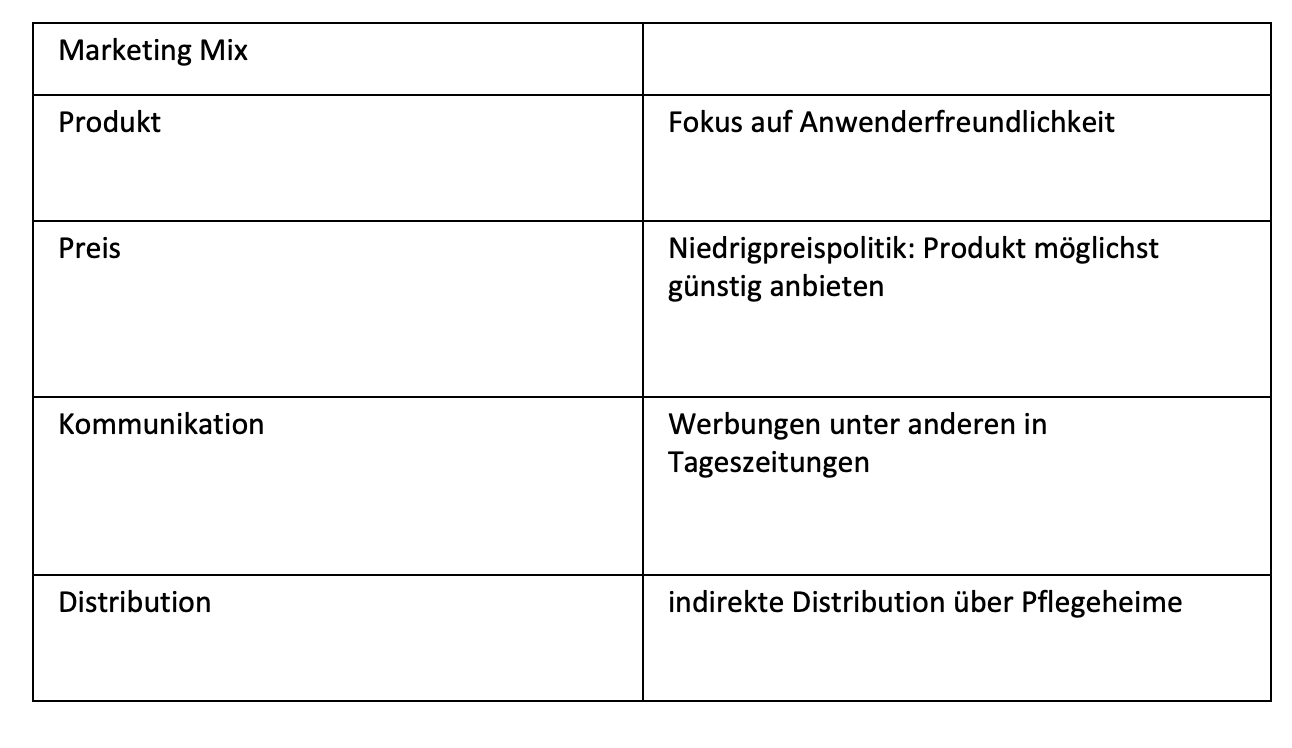
\includegraphics[width=8cm]{Marketing_Mix.png}
         \caption{Marketing Mix}
         \label{fig:Marketing_Mix}
        \end{figure}
        
         \begin{figure}[h]
         \centering
         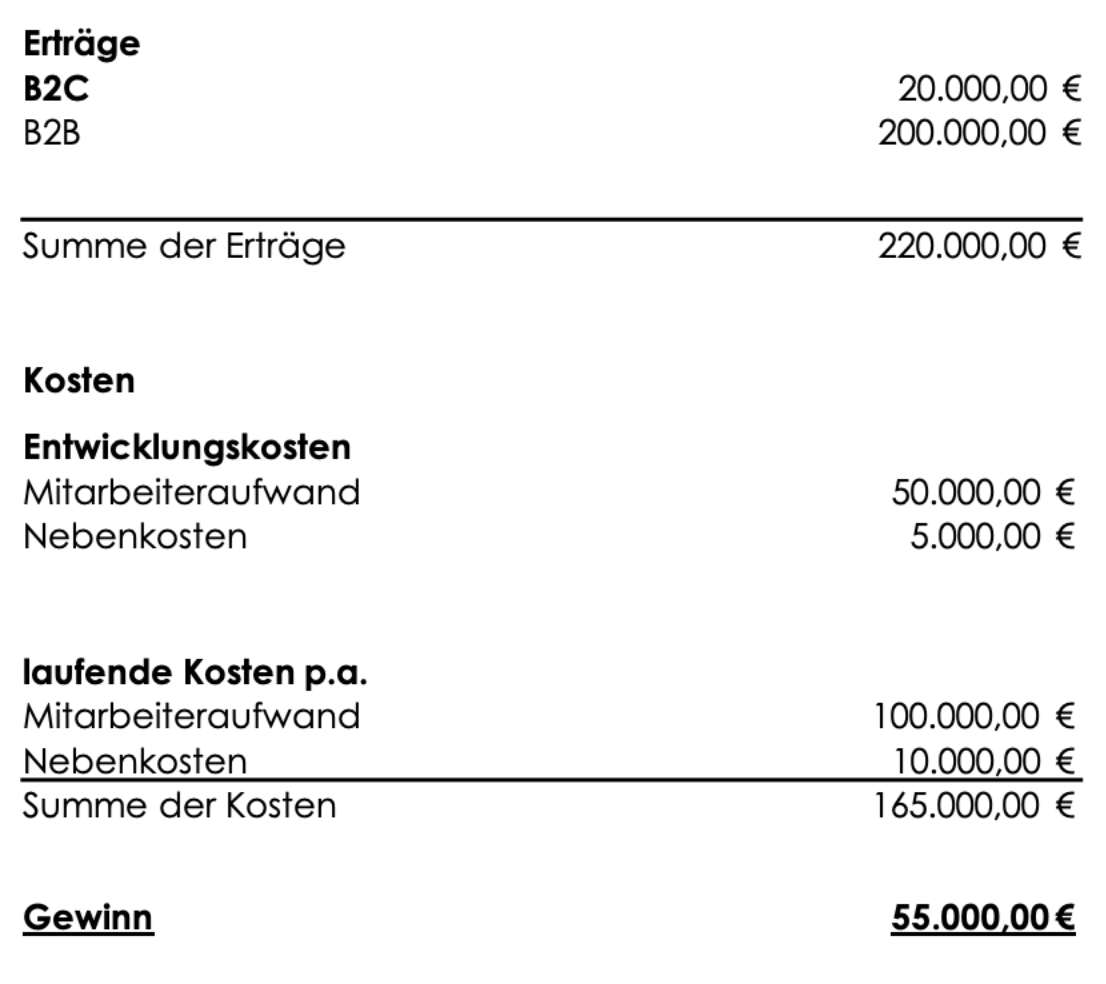
\includegraphics[width=8cm]{Ertrag_Jahr01.png}
         \caption{Laufende Kosten/Erträge & Entwicklungskosten }
         \label{fig:Ertrag_Jahr01}
        \end{figure}
         
         \begin{figure}[h]
         \centering
         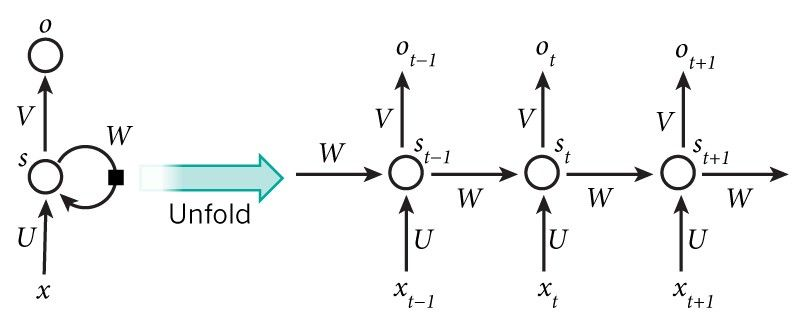
\includegraphics[width=8cm]{rnn.jpg}
         \caption{Funktionsweise eines Recurrent Neural Networks}
         \label{fig:rnn}
        \end{figure}
        
         \begin{figure}[h]
         \centering
         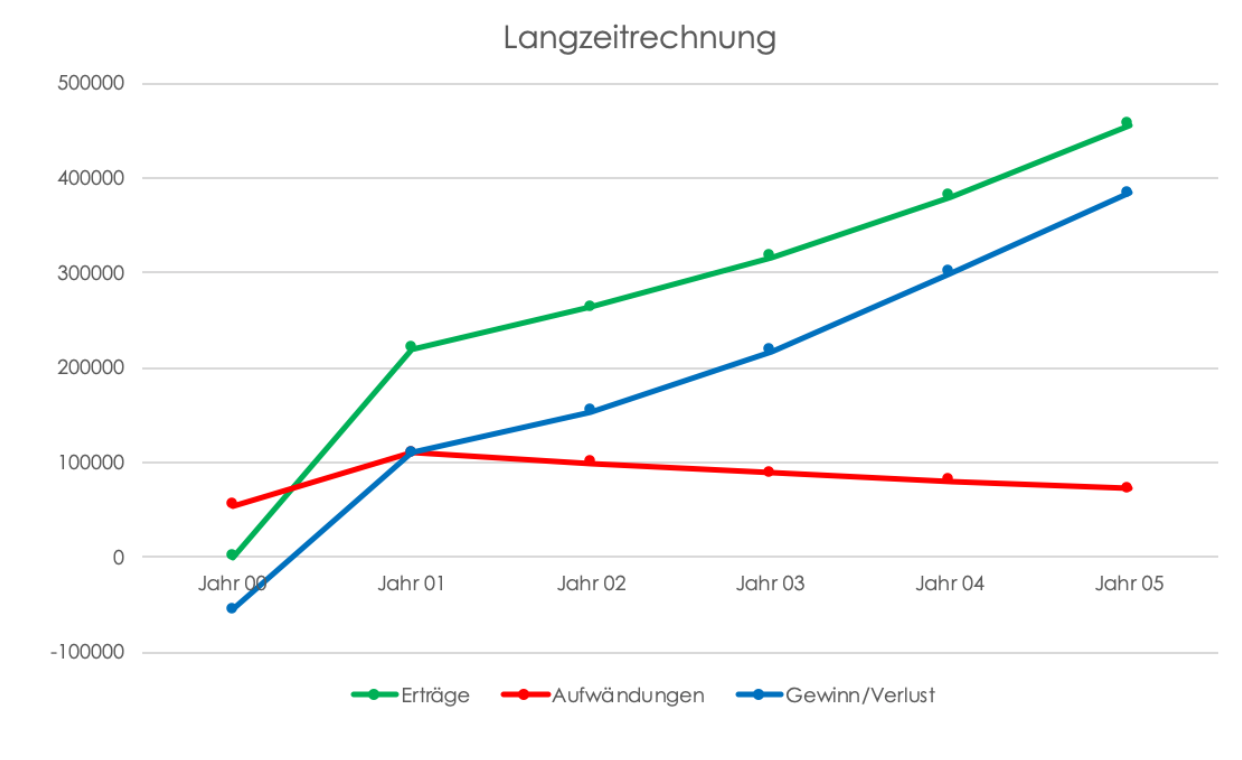
\includegraphics[width=8cm]{Langzeitertrag.png}
         \caption{Langzeitertrag}
         \label{fig:Langzeitertrag}
        \end{figure}
         
         \begin{figure}[h]
         \centering
         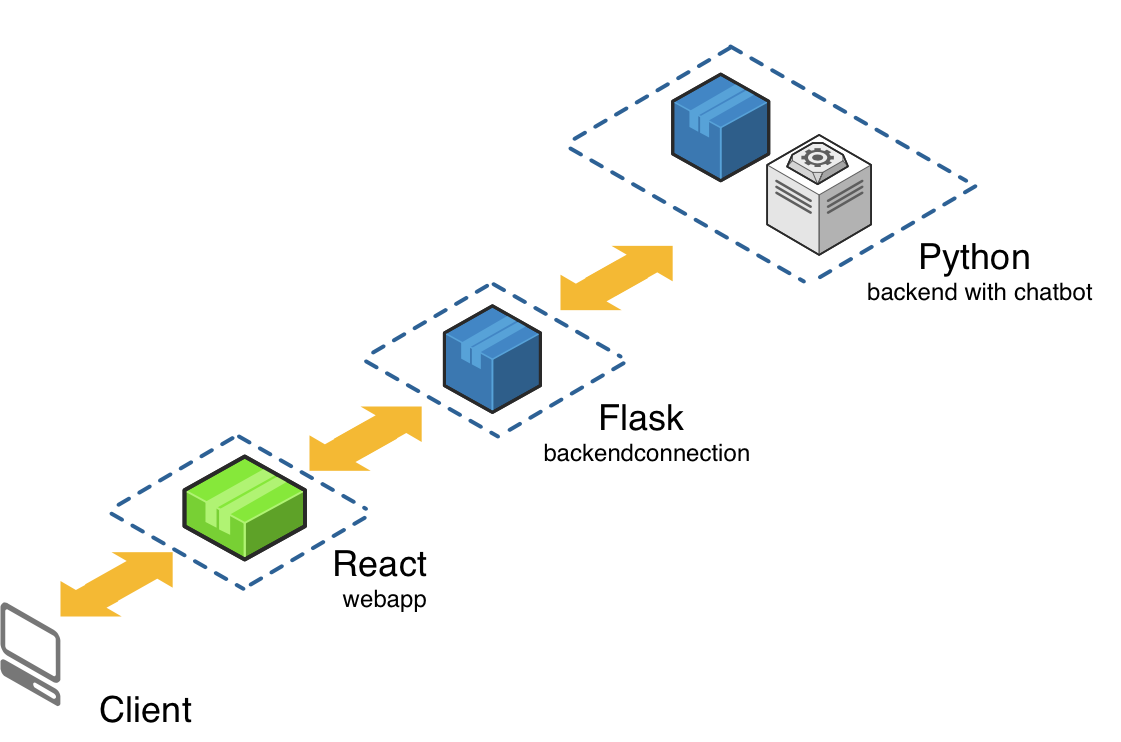
\includegraphics[width=8cm]{systemarchitektur_v2.png}
         \caption{Systemarchitektur}
         \label{fig:Systemarchitektur}
        \end{figure}
        
        \begin{figure}[h]
         \centering
         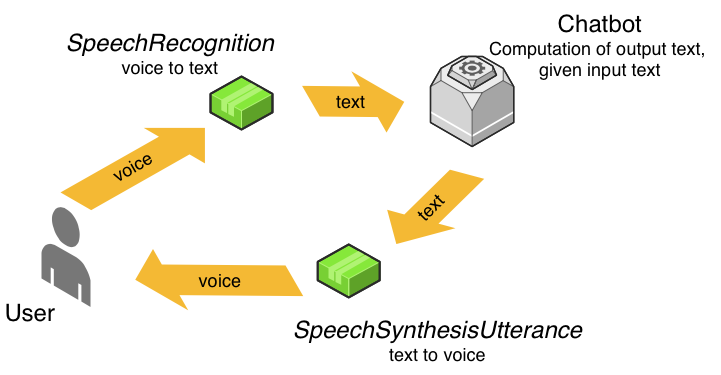
\includegraphics[width=8cm]{voice_v2.png}
         \caption{Sprachverarbeitung}
         \label{fig:Sprachverarbeitung}
        \end{figure}
        
        \begin{figure}[h]
         \centering
         \includegraphics[width=8cm]{Lstm.png}
         \caption{LSTM Encoder und Decoder}
         \label{fig:lstm}
        \end{figure}
        
        \begin{equation}
         \nametag{Similarity =}\\
         \frac{\sum_{i=1}^{n} a_i \cdot b_i}{\sqrt{\sum_{i=1}^{n} (a_i)^2} \cdot \sqrt{\sum_{i=1}^{n} (b_i)^2}} 
        \label{eq:similarity}
        \end{equation}
        
        \begin{figure}[h]
         \centering
         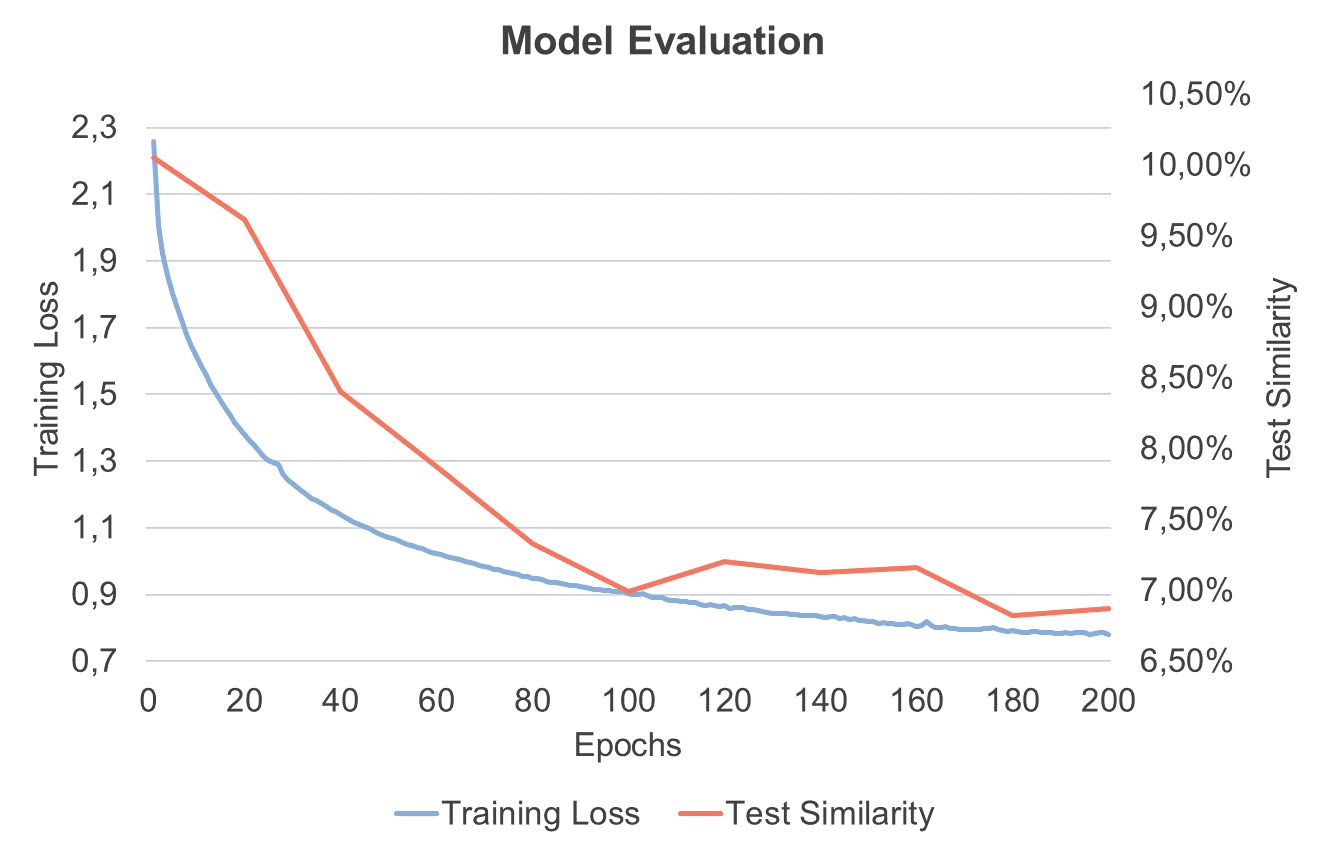
\includegraphics[width=8cm]{model_evaluation.png}
         \caption{Trainings- und Testergebnisse der Modelle}
         \label{fig:model}
        \end{figure}



% WARNING
%-------------------------------------------------------------------
% Please note that we have included the references to the file aa.dem in
% order to compile it, but we ask you to:
%
% - use BibTeX with the regular commands:
%   \bibliographystyle{aa} % style aa.bst
%   \bibliography{Yourfile} % your references Yourfile.bib
%
% - join the .bib files when you upload your source files
%-------------------------------------------------------------------

\begin{thebibliography}{}

  \bibitem[Bird(2009)]{bird} Bird, Steven; Klein, Ewan; Loper, Edward. 2009, Natural Language Processing with Python (O'Reilly Media Inc, Sebastopol) 504
  
  \bibitem[Aunt Elisa (2020)]{auntelisa} Deufel Johannes; Fischer, Jannik; Marx, Simone; Scapan, Simon. 2020, README.md. (Project Aunt Elisa) URL: https://github.com/SimonScapan/AuntElisa (Zugriff: 12.07.2020)
    
  \bibitem[Goyal(2018)]{goyal} Goyal, Palash; Jain, Karan; Pandey, Sumit. 2018, Deep Learning for Natural Language Processing: Creating Neural Networks with Python (Apress, Berkeley) 277
  
  \bibitem[Hasani (2020)]{hasani} Hasani, Moein. 2020, Chatbot-with-TensorFlow-and-Keras. (GitHub) URL: https://github.com/Moeinh77/Chatbot-with-TensorFlow-and-Keras (Zugriff: 05.07.2020)
  
  \bibitem[Heidenreich (2019)]{heidenreich} Heidenreich, Hunter. 2019, Understanding Keras — Dense Layers. (medium) URL: https://medium.com/@hunterheidenreich/understanding-keras-dense-layers-2abadff9b990 (Zugriff: 14.07.2020)
    
  \bibitem[Jackson (2020)]{jackson} Jackson, Christy; Nawas, Khadar; Prassanna, J.; R. Parabakaran; Ramanath, Sakkaravarthi. 2020, Towards Building A Neural Conversation Chatbot Through Seq2Seq Model. In: International journal of scientific & technology research. Volume 9 (Nextgen) 1219 - 1222
  
  \bibitem[Koehrsen (2018)]{koehrsen} Koehrsen, Will. 2018, Recurrent Neural Networks by Example in Python. (towards data science) URL: https://towardsdatascience.com/recurrent-neural-networks-by-example-in-python-ffd204f99470 (Zugriff: 02.07.2020)
  
  \bibitem[Kostadinov (2017)]{kostadinov} Kostadinov, Simeon. 2017, Understanding GRU Networks. (towards data science) URL: https://towardsdatascience.com/understanding-gru-networks-2ef37df6c9be (Zugriff: 14.07.2020)  
  
  \bibitem[Kumar (2018)]{kumar1} Kumar, Aditya. 2018, Chatbot Development using Deep Learning & NLP implementing Seq2Seq Model. (Medium) URL: https://medium.com/analytics-vidhya/chatbot-development-using-deep-learning-nlp-implementing-seq2seq-model-eb1114903523 (Zugriff: 02.07.2020)
  
  \bibitem[Kumar (2019)]{kumar2} Kumar, Dilip; Rajpoot, Gaurav; Sehrawat, Monica; Srivastava, Arul. 2019, Chatbot using Deep Learning (Seq2Seq Models). In: International journal of scientific & technology research. Volume 5 (Nextgen) 18 - 21
  
  \bibitem[Mozilla (2019)]{mozilla19} Mozilla Developer Network. 2019, SpeechSynthesis. (MDN web docks) URL: https://developer.mozilla.org/de/docs/Web/API/SpeechSynthesis (Zugriff: 02.07.2020) 
  
  \bibitem[Mozilla (2020)]{mozilla20} Mozilla Developer Network. 2020, SpeechRecognition. (MDN web docks) URL: https://developer.mozilla.org/en-US/docs/Web/API/SpeechRecognition (Zugriff: 02.07.2020)
  
  \bibitem[Takezawa (2019)]{takezawa} Takezawa, Akira. 2019, How to implement Seq2Seq LSTM Model in Keras #ShortcutNLP. (towards data science) URL: https://towardsdatascience.com/how-to-implement-seq2seq-lstm-model-in-keras-shortcutnlp-6f355f3e5639 (Zugriff: 02.07.2020)

  \bibitem[Tensorlayer (2019)]{tensorlayer} Tensorlayer. 2019, Seq2Seq Chatbot. (GitHub) URL: https://github.com/tensorlayer/seq2seq-chatbot (Zugriff: 28.06.2020)
  
  \bibitem[Venkatachalam (2019)]{venkatachalam} Venkatachalam, Mahendran. 2019, An introduction to Attention. (towards data science) URL: https://towardsdatascience.com/an-introduction-to-attention-transformers-and-bert-part-1-da0e838c7cda (Zugriff: 14.07.2020)

\end{thebibliography}

\end{document}